\documentclass[a4paper,fleqn]{cas-sc}

 %\usepackage[numbers]{natbib}
%\usepackage[authoryear]{natbib}
%\usepackage[authoryear,longnamesfirst]{natbib}
\usepackage{float}
\usepackage{svg} 
\usepackage[utf8]{inputenc}
%\usepackage{fontspec}
%\newfontface{\bn}{kalpurush.ttf} 
\usepackage[numbers]{natbib}
\usepackage{tabularx}
\usepackage[english]{babel} 
\usepackage{algorithm} 
\usepackage{algpseudocode}
\usepackage{lineno}
\usepackage{amsmath}
\usepackage{amsfonts}
\usepackage{amssymb}
\usepackage{algpseudocode} 
\usepackage{booktabs}
\usepackage{multirow} 
\usepackage{changepage} 
\usepackage{orcidlink}
\usepackage{hyperref}
\usepackage{subcaption}
\usepackage{color}
\usepackage{xcolor} 
%%%Footer and ORCID adjustments
% This is a preprint, not a submitted manuscript: drop the "submitted to Elsevier" wording.
\ExplSyntaxOn
\cs_set:Npn \__first_footerline:
  {
    \group_begin:
    \small
    \sffamily
    \ifnum\theblind>0\relax
    \else
    \__short_authors: :~
    \fi
    \rmfamily \itshape Preprint
    \group_end:
  }
\ExplSyntaxOff
% No ORCID identifiers are used, so hide the empty ORCID footnote.
\RenewDocumentCommand \printorcid { } { }
%%%Author definitions
\def\tsc#1{\csdef{#1}{\textsc{\lowercase{#1}}\xspace}}
\tsc{WGM}
\tsc{QE}
\tsc{EP}
\tsc{PMS}
\tsc{BEC}
\tsc{DE}
%%%
%\rightlinenumbers*
\begin{document}
\let\WriteBookmarks\relax
\def\floatpagepagefraction{1}
\def\textpagefraction{.001}

% Short title
\shorttitle{Trust-Calibrated Multi-Agent Scientific Deliberation for Mitigating Sycophantic Consensus}

% Short author
\shortauthors{Rahaman et~al.}

% Main title of the paper
\title [mode = title]{Trust-Calibrated Multi-Agent Scientific Deliberation for Mitigating Sycophantic Consensus in LLM Reasoning}


\author[1]{Md. Atikur Rahaman}
\cormark[1]
\ead{mrahaman2310298@bscse.uiu.ac.bd}
\credit{ Conceptualization, Formal analysis,  Methodology, Writing-original draft, Writing-review \& editing}
% Address/affiliation
\affiliation[1]{organization={Computer Science and Engineering, United International University},
  %addressline={}, 
  city={Dhaka},
  citysep={}, % Uncomment if no comma needed between city and postcode
  postcode={1212},
  %state={E Wesley Ave, Denver},
  country={Bangladesh}}

% Second author
\author[1]{Rakibul Hasan}
\ead{rhasan2310530@bscse.uiu.ac.bd}
\credit{Conceptualization, Data curation, Formal analysis, Methodology, Validation}

% Third author
\author[1]{Md. Salman Rohoman Nayeem}
\ead{salmanrahman339@gmail.com}
\credit{Data curation, Investigation, Software, Writing - review \& editing}

% Fourth author
\author[1]{Pratay Paul}
\ead{ppaul2310163@bscse.uiu.ac.bd}
\credit{Data curation, Software, Validation, Visualization}

% Fifth author
\author[1]{Yousuf Kamal Himel}
\ead{yhimel2310526@bscse.uiu.ac.bd}
\credit{Data curation, Formal analysis, Validation, Writing - review \& editing}

% Sixth author
\author[1]{Mst. Farjana Akter Limu}
\ead{mlimu2310535@bscse.uiu.ac.bd}
\credit{Data curation, Software, Validation, Visualization}

% Supervisor
\author[1]{Mohammad Nurul Huda}
\credit{Investigation, Supervision, Visualization}

% FYDP faculty
\author[1]{Ohidujjaman}
\credit{Supervision, Validation, Writing - review \& editing}

\cortext[cor1]{Corresponding author: Md. Atikur Rahaman (mrahaman2310298@bscse.uiu.ac.bd)}

% Here goes the abstract
\linenumbers
\begin{abstract}
  Large language models have done surprisingly well at answering many scientific questions. However, large language models also continue to "hallucinate" and reason incorrectly. One potential solution to these problems is multi-agent debate. Although a correct minority may exist, a confident but incorrect majority can drag this correct minority agent down and lead the group to select the wrong answer. This is known as the "sycophantic consensus." Currently, there is no mechanism within any debate system to check an individual agent's assertions against outside scientific evidence before allowing them to gain influence in the debate. Instead of using a simple vote-weighted approach, we intend to assign a trust score to every participating agent based on how much scientific evidence supports their responses. Every time agents respond during a round, the system breaks down their responses into small units of factually verifiable statements ("claims"). After breaking down the response, the system locates all relevant scientific literature that could support or contradict each claim. Because unsupported claims eventually lose influence and because the trust scores are kept in bounds, the probability increases that a correct minority will survive long enough to ultimately win. Our proposed framework produced fewer hallucinated answers than competing frameworks because all surviving claims are linked back to their originating passages of scientific evidence. To test this hypothesis, we compare our proposed framework to majority voting and other baseline systems. Once all models have finished responding to a given question, the system returns both the selected model and supporting citations for that model. The performance of our proposed framework is evaluated via four metrics: answer accuracy, consensus collapse, minority preservation, and evidence calibration.

\end{abstract}
% Keywords
% Each keyword is separated by \sep
\begin{keywords}
  Large language models \sep Multi-agent debate \sep  Retrieval-augmented generation \sep  Sycophancy \sep Scientific question answering \sep Trust calibration
\end{keywords}

\maketitle
\linenumbers
\section{Introduction}\label{sec1}

Large language models are capable of answering scientific questions in a way that could make them useful for tutoring and supporting decisions. However, even though a model may be fluent in its language, it can still provide an answer based on false premises or assumptions. The use of multi-agent debate will reduce the risk of providing incorrect information. There are three agents who are all responding to the same question and debating one another’s reasoning over multiple rounds~\cite{du2024improving}. In addition, chain-of-thought prompting allows users to see how each model arrives at an answer and what steps were taken to arrive at that answer~\cite{wei2022chain}. The weakness lies in the final round of the debate. Most systems use some type of majority vote to determine which answer(s) prevail. Each agent has equal weight and the response receives credit if it represents the majority response ~\cite{wang-etal-2024-rethinking-bounds}. As a result, when there is a clear and confident wrong answer, there is nothing to prevent the winning minority agent from dropping their answer due to the confidence exhibited by the wrong answer; therefore, both parties are recorded as having agreed on the wrong response~\cite{choi2025debate}. When this occurs, it is referred to as sycophantic consensus~\cite{pitre-etal-2025-consensagent}.  Yao et al. formalize inter-agent sycophancy in multi-agent debate and show that it collapses disagreements into premature consensus before the correct answer is reached~\cite{yao2025peacemaker}. Sharma et al. identify the propensity for preference training, which trains models to accept plausible positions ~\cite{sharma2024sycophancy}. NO current debate system verifies an agent's claims using outside sources of scientific evidence prior to granting that agent influence. This study creates a trust-calibrated multi-agent deliberation framework to address this void. Each agent's answer is split into small factual claims. The claims are checked against retrieved scientific literature, and every agent holds a bounded trust score that rises with supporting evidence and falls with contradicting evidence. The final answer comes from trust-weighted aggregation instead of a head count. The method is tested on GPQA and MMLU-Pro, and it needs no fine-tuning because all models run as served inference.

Du et al. show that debate improves factuality and reasoning over a single pass, but their agents are treated equally and their claims are never checked against external sources~\cite{du2024improving}. Pitre et al. report that the correct answer is present in the discussion yet ignored in more than 20 percent of wrong-answer cases, and their prompt-rewriting fix still leaves the final decision on self-reported confidence~\cite{pitre-etal-2025-consensagent}. Yoffe et al. use re-weight agents based upon token level signals and their ground truth experiment limits how much a model can improve upon that signal~\cite{yoffe-etal-2025-debunc}. ReConcile pools together multiple different models and then weight each of them based upon their estimated confidence internally~\cite{chen2024reconcile}. Fan et al. target the token cost of debate with a classifier that decides whether a debate is needed at all~\cite{fan2026imad}. Sparse topology reduces communication Cost, but doesn’t reduce the overall Cost associated with aggregating ~\cite{li-etal-2024-improving-multi}. Wang et al. pool together many different models using static aggregation and perform well on open benchmark data, but there was no per-agent trust or evidence checking ~\cite{wang2025mixture}. Diversity and training time methods change how agents reason not how much each agent’s vote counts in final answer ~\cite{liu2025breaking,subramaniam2025multiagent}. Intervention testing shows that most sycophancy fixes are not enough on their own to be successful~\cite{wynn2025talk}. He et al. find a previously correct minority being suppressed after a debate and they reverse the majority, however, the reversal occurs too late to save the minority while they continue to argue ~\cite{he2026minority}.

In all of these systems the amount of influence each agent has is determined by either a vote or an internal score; however, none of the systems evaluate an agent's claims against evidence while the debate is occurring. Using an agent's self reported confidence as a measure is inadequate since training models to be agreeable also trains them to be sycophantic~\cite{ibrahim2026training}, and alignment experiments show that agreeing with wrong user positions increases after fine-tuning ~\cite{chen2025self}. Theory states that agents will converge toward a wrong majority unless some form of outside correction enters into the loop ~\cite{estornell2024multillm}, and multi-agent systems fail in recurring ways that diagnosis alone does not fix~\cite{cemri2025why}. Surveys have mapped the design space and its challenges~\cite{li2024survey}. Some applied variants of debate adapt it to grounded reasoning about knowledge~\cite{wang2025learning} and scientific code generation~\cite{wang2025scalability}, while other researchers studied research ideation~\cite{ueda2025exploring}, educational reasoning~\cite{zhou2025adaptive}, and communications engineering~\cite{gomez2026multiagent}. This study ties the amount of influence each agent has to external evidence during the debate. Claims are evaluated against retrieved passage from science sources~\cite{karpukhin2020dense}, in line with work that grounds correction in external tools~\cite{gou2024critic} and studies that report factual gains due to knowledge-grounded correction~\cite{yang2025comprehensive}.  The trust score is bounded so no one agent can be silenced or made all-powerful; the final decision uses those weights. Scientific question sets provide a suitable testbed because they carry verifiable answers and published literature that retrieval can access; gpqa and MMLU-pro provide for comparison against established baseline results. Outcome provides a reproducible framework that reduces consensus collapse, preserves a correct minority more often than previous methods, maintains stable accuracy rates for answers, and provides a calibrated trust signal.

%%%%%%%%%%%%%%%%%%%%%%%%%%%%%%%%
\section{Conventional Method}\label{sec2}

\subsection{Preliminaries}

Large language models are able to generate responses for scientific questions with high levels of confidence; however, large language models still produce confident errors. Chain-of-thought prompting provides the rationale or reasoning process behind the generated response, therefore allowing the end-user (reader) to understand how the response was developed~\cite{wei2022chain,zhang2025from}. Multi-Agent Debate extends chain-of-thought prompting. Multiple agents respond to a question, examine the rationale of another agent's reasoning, and modify their position based upon a multi-round dialogue prior to producing a final response~\cite{du2024improving}. As much emphasis needs to be placed on the aggregation of multiple agent responses as is necessary when examining individual agent reasoning processes. In most cases, debate systems combine agent responses using a simple majority voting system where all agents have equal weighting in the voting process~\cite{choi2025debate}. Majority voting systems count repeated responses. They do not verify if any single response produced by an agent is accurate. Therefore, even though some agents may possess a minority view based upon incorrect assumptions and confidence, if there are enough agents who provide repeated responses agreeing with the incorrect assumptions, they will influence one or more additional agents to agree with them. Once the vote is recorded, the resulting output is considered as ``agreement'', which is referred to as consensus~\cite{pitre-etal-2025-consensagent}. Confidence within the answers provided by a debate system typically depends on two types of confidence signals: Self-Reported Confidence and Token-Level Uncertainty. However, neither signal verifies if the claim made is accurate~\cite{yoffe-etal-2025-debunc}. Therefore, trust within the answers produced by a debate system must arise from evidence external to the debate system itself.


\subsection{Existing Methods}

The work done previously addresses some of these issues. In terms of existing approaches that could be used to solve these problems, Du et al. have shown that debating improves the performance (in terms of factuality and reasoning) over a single run. However, there was an assumption made in their approach that all of the agents are treated similarly and their statements were never cross-checked against external data~\cite{du2024improving}. Also, Fan et al. reduced the cost of debate with a classifier that predicts whether a debate is worthwhile from the structured self-critique of a single agent, so easy questions skip the debate entirely. The debate itself continued to use a majority vote process to determine what the output of the debate should be once it began~\cite{fan2026imad}. Wang et al. showed how combining multiple different models into a pipeline using a layering process produces good results on public benchmarks. They did not perform any form of trust evaluation with respect to individual agents nor did they perform any type of evidence checking~\cite{wang2025mixture}. Zhou et al. demonstrated how specialized agents may be selected for specific tasks via a reward-based methodology. This selection process determines which agent will be assigned to do a particular task; however, the amount of weight given to each agent's response is not evaluated~\cite{zhou2025reso}.

There exists another set of methodologies that attempt to mitigate sycophancy directly. A first example is provided by Pitre et al., who found that the correct answer existed within the discussion but was ignored greater than twenty percent of times that the agent produced an incorrect answer~\cite{pitre-etal-2025-consensagent}. The methodology employed by Pitre et al. included detecting instances of either stalling or copy-and-paste behavior by the agents. Once detected, the methodology re-wrote the original task prompt and caused the debate to be restarted. However, although the methodology attempted to detect and eliminate sycophantic behavior, ultimately a vote among the participating agents was still taken using self-reported confidence values~\cite{pitre-etal-2025-consensagent}. Another example is provided by Chen et al., who demonstrated how sycophancy may be reduced through aligning preferences between models at training time. Although this methodology may be effective at reducing sycophancy in some settings, it only addresses sycophancy for a single model and does not provide any means to address sycophancy in a live debate setting~\cite{chen2025self}. An additional example is provided by Ibrahim et al., who demonstrated that training models to produce responses that appear friendly reduces factual accuracy and increases agreement with false beliefs held by users~\cite{ibrahim2026training}. Finally, an additional example is provided by He et al., who demonstrated that post-debate, it is possible to detect and correct a minority of participants whose answers were initially suppressed. Additionally, He et al. also demonstrated how flipping the decision made by the majority may correct previous mistakes made during the rounds; however, this detection occurs too late to prevent the suppression of minority opinions during the debate rounds~\cite{he2026minority}.

Finally, there exist methodologies that modify the information available to agents prior to a debate. For example, Yoffe et al. proposed a mechanism whereby token-level uncertainty may be applied to weigh influence of agents during the course of a debate. Using this methodology, the authors of Yoffe et al. conducted experiments where they used actual ground truth to demonstrate that the gain achieved using this methodology is limited by quality of internal signal~\cite{yoffe-etal-2025-debunc}. As a second example, Gou et al. grounded corrections in external tools for use with a single agent~\cite{gou2024critic}. As a third example, Kushwaha and Madhavan identified discrepancies between passages returned by search engines and scored credibility of sources prior to generation, without engaging in debate between agents~\cite{kushwaha2026agentbased}. As a fourth example, Karpukhin et al. developed the dense passage retrieval algorithm that is being used in this study for retrieval phase~\cite{karpukhin2020dense}.

Finally, theory and analysis of mechanisms provide remaining examples. Estornell and Liu proved that similar responses result in majority tyranny and that sharing misconceptions amongst agents decreases accuracy as more agents become aware of those same misconceptions~\cite{estornell2024multillm}. Choi et al. separated debate from voting and demonstrated that majority voting accounts for most of the improvement usually credited to debate, with debate rounds adding little once votes are aggregated~\cite{choi2025debate}. Cui et al. removed consensus requirement and scored debate trajectory instead~\cite{cui2026freemad}. Pitre et al. studied quality of processes involved in debates when ground truth cannot be obtained~\cite{pitre2026diagnostic}. Cemri et al. constructed failure taxonomy for multi-agent systems and reported failure rates ranging from 41% to 86.7% across seven systems. Ultimately, Cemri et al. left correction for future studies~\cite{cemri2025why}. Cau et al. demonstrated that selective persuasion leads to increased agreement. Similarly, Yeow et al. demonstrated how feedback between agents can rapidly propagate early errors~\cite{cau2025selective,yeow2025reliable}.


\subsection{Research Gap}

There are three areas that have yet to be resolved with multi-agent debate. First, there is the question of the cost associated with debating. In terms of using tokens (i.e., money) to pay for debates, iMAD is able to predict if a debate will need to occur prior to the start of the debate and therefore reduces costs for simple questions~\cite{fan2026imad}. Second, there is the problem of determining whether two agents are agreeing due to either conformity or sycophancy. CONSENSAGENT identifies instances where agents may ``stall'' or copy answers, and it then changes the prompt prior to the next round~\cite{pitre-etal-2025-consensagent}. Third, there is the question of how to determine which agent should have greater influence when agents disagree. DebUnc attempts to use self-reported uncertainty as the basis upon which to weigh agent influence; however, its own experimental evaluation indicates that only the quality of the uncertainty signal received affects how well the weighting mechanism performs~\cite{yoffe-etal-2025-debunc}.

Currently available solutions do not resolve the third area. Static aggregation treats each proposer equally and provides a synthesis based upon the output from one model, thereby providing a confident incorrect proposer with equal status in the production of the final answer~\cite{wang2025mixture}. Process-level diagnosis determines whether a debate is healthy, but it does not affect the decision itself~\cite{pitre2026diagnostic}. After the conclusion of a debate, a post-hoc flip could provide some protection to a previously suppressed minority; however, the pressure placed upon that minority occurs at the time of the debate, not after~\cite{he2026minority}. Furthermore, tool-based correction involves verifying the output from one agent in isolation and does not facilitate arbitration between different agents~\cite{gou2024critic}. Additionally, retrieval-side credibility scoring allows for ranking of sources prior to a single generation pass and includes no revision rounds nor consideration of agent trust~\cite{kushwaha2026agentbased}. Theory predicts that agents who rely on others for information tend to follow the opinions of the majority regardless of their correctness, and further theory suggests that sharing errors among multiple agents results in reduced accuracy as those errors are amplified through the number of agents involved~\cite{estornell2024multillm}. Studies conducted at training-time demonstrate that alignment increases this phenomenon since models that are trained to produce responses that are perceived as cooperative become more likely to engage in behaviors that are seen as sycophantic and less likely to generate accurate responses~\cite{ibrahim2026training,chen2025self}. Finally, empirical studies of failure indicate that these types of failures are both common and identifiable and leave resolution of these failures to subsequent research~\cite{cemri2025why}.

In all of the reviewed literature, influence is determined via a vote, a self-reporting score, a rewritten prompt, or a post-hoc flip. None of the methods employed thus far involve verifying an agent's claim against independent evidence while a debate is occurring, and none employ such verification in order to determine what weight an agent should receive in making a final determination. Therefore, this paper addresses this gap with a bounded trust score that is updated from retrieved evidence throughout the course of a debate and used for the final aggregation.


\section{Proposed Method}\label{sec3}

\subsection{Overview of Framework}
This is a deliberation layer placed in the middle of an original question and its solution. Once you've passed through the confidence gate, your question will either be answered directly or sent to a full debate. In a debate there are three independent heterogeneous agents answering your question and tagging all claims made during their reasonings. Every single claim tagged from their reasoning's are then cross-checked using the scientific evidence that has been retrieved. After they have finished cross-checking their respective claims with scientific evidence, the verdict of the cross checking process will affect the trust score of each individual agent. At this point the agents will revise their position based on what they believe about other agents' positions as well as their own trust scores. This loop can run no longer than 3 times. Based on their respective trust scores and positions, the final answer is determined via a weighted average of the positions of the agents. The package containing your results include; the answer to your question, the citations that support the answer to your question, the trust trajectory, and the reasoning trace of each of the agents involved.Figure~\ref{fig:framework-flow} shows the end-to-end flow, and Figure~\ref{fig:context} shows the system boundary and the external actors.

\begin{figure}[pos=htbp]
  \centering
  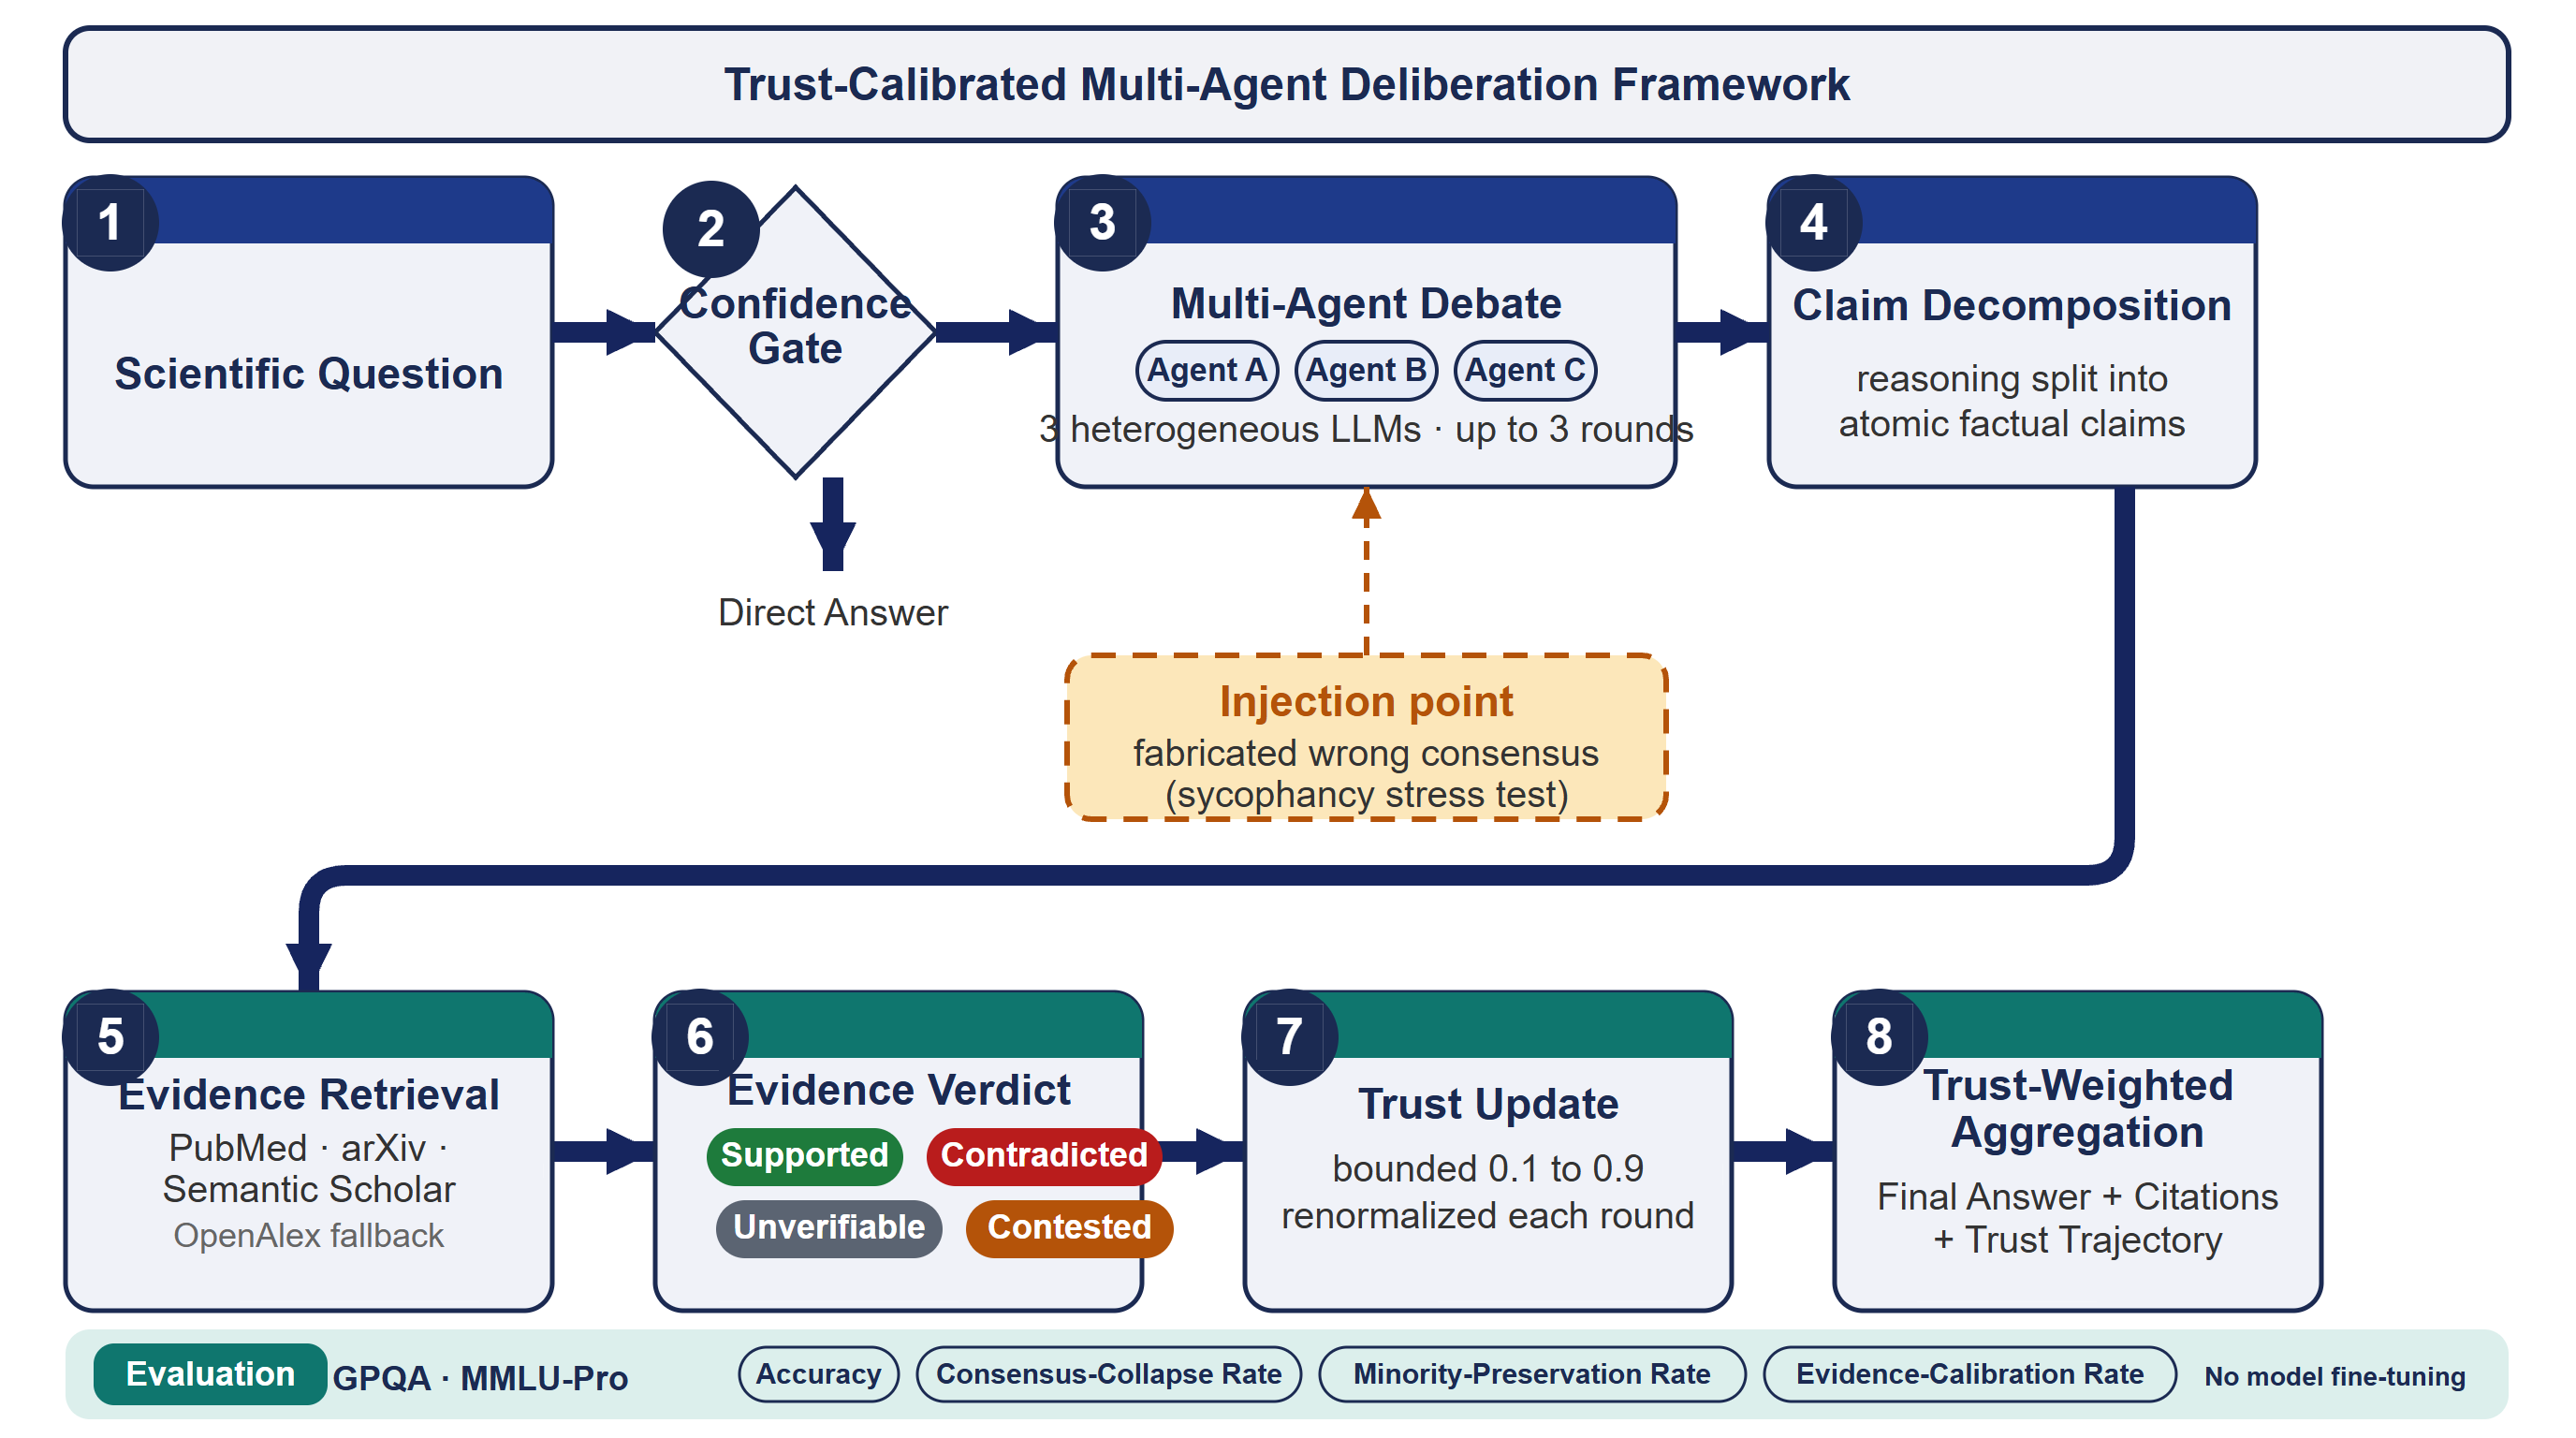
\includegraphics[width=0.88\linewidth]{fig-pipeline.png}
  \caption{End-to-end flow of the trust-calibrated multi-agent deliberation framework: debate, claim-level evidence verification, per-round trust updates, and trust-weighted aggregation.}\label{fig:framework-flow}
\end{figure}

\begin{figure}[pos=htbp]
  \centering
  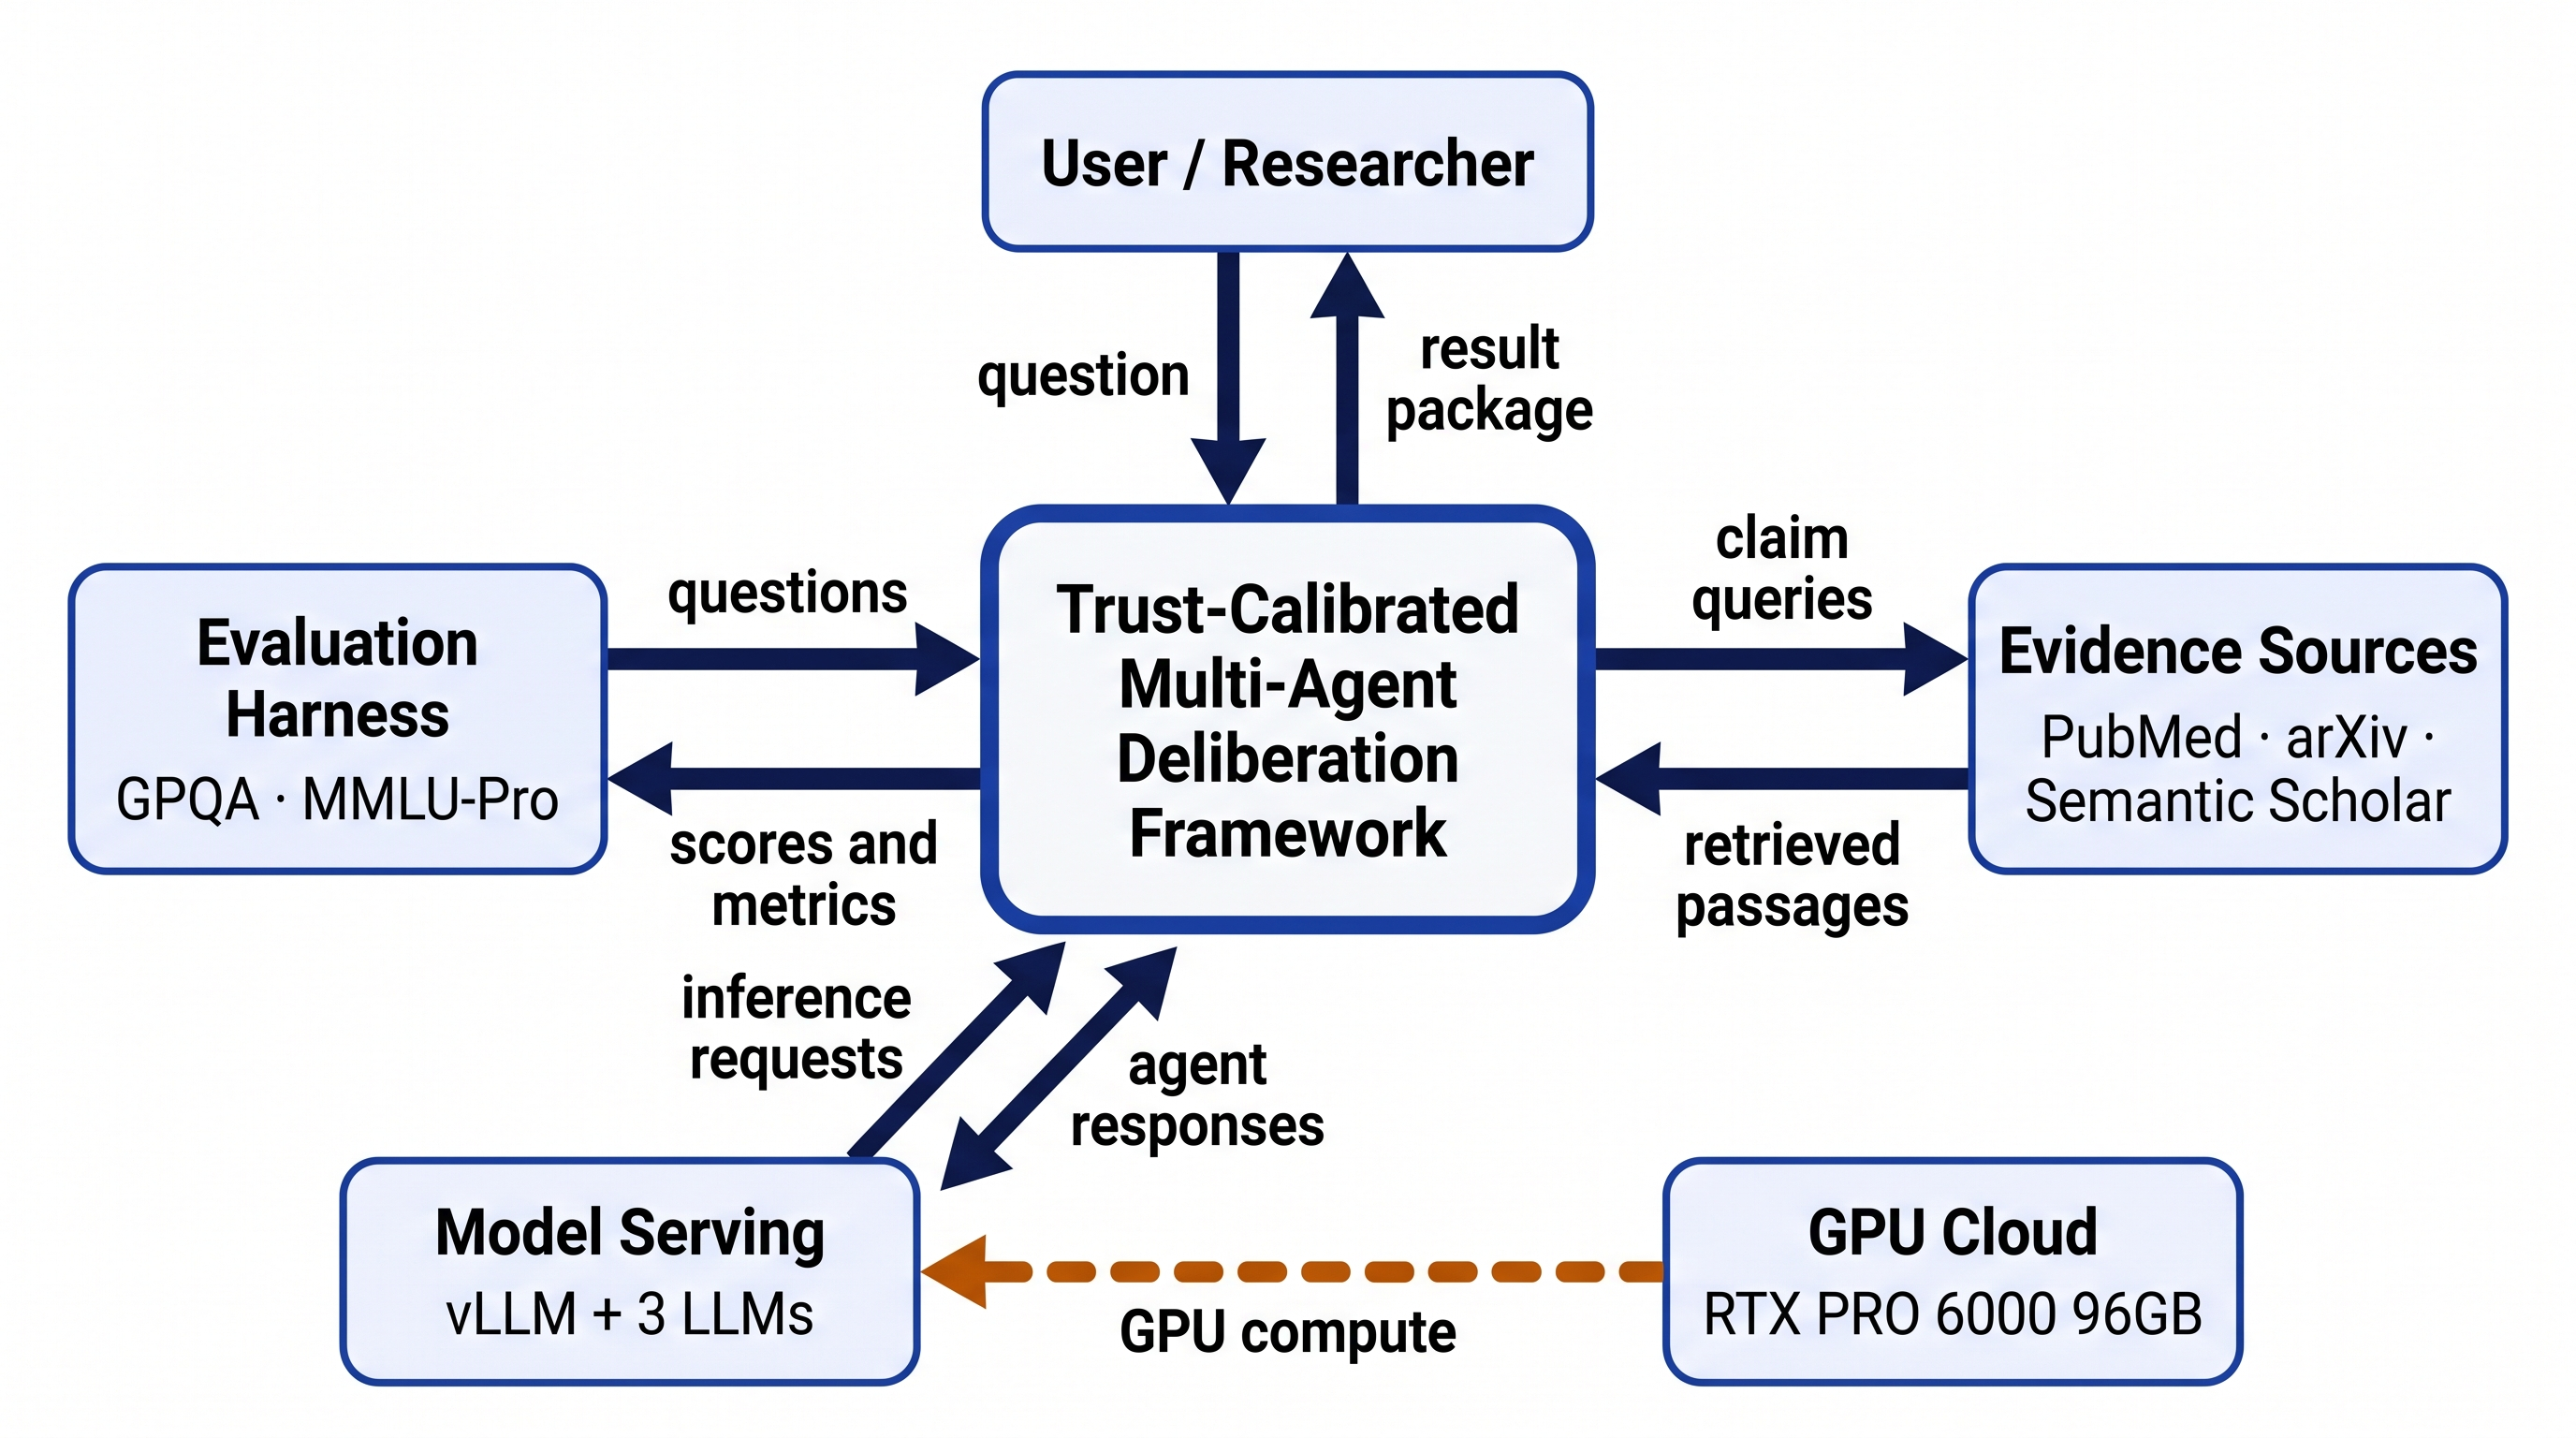
\includegraphics[width=0.80\linewidth]{fig-context.png}
  \caption{Context diagram of the framework. The evaluation harness submits questions, the evidence sources return passages, the model server runs the three agents, and the user receives the result package.}\label{fig:context}
\end{figure}

\subsection{Confidence Gate}
The gate keeps the cost low on easy questions. One agent answers the question with a short chain of thought and reports a confidence value, or three quick agent calls answer the same question and the gate compares the answers. A low confidence or a disagreement sends the question to the full pipeline. A high confidence sends the question to a direct answer. The gate affects throughput and not the core evaluation, because the evaluation set keeps only questions that produce divergent initial answers.

\subsection{Heterogeneous Debate Agents}
Three agents answer the question in round zero. Each agent is a different model family, so the agents do not share the same training data and the same blind spots~\cite{estornell2024multillm}. The development configuration uses Qwen3.5-9B, Gemma 4 12B, and Ministral-3-14B-Instruct-2512. The final configuration replaces them with Qwen3.6-27B, Gemma 4 26B A4B, and Mistral-Small-3.2-24B-Instruct-2506. All models are served through vLLM behind an OpenAI-compatible interface, and no model is fine-tuned. Each agent produces an answer, a reasoning trace, and a list of tagged claims in the form \texttt{<claim id="c1">}. The tags make claim-level checking possible in later stages.

\subsection{Claim Decomposition}
A compound sentence can carry more than one fact. The decomposition step splits each agent answer into small factual statements, and every statement keeps the identifier of its source agent. A schema check validates the tagged output. A failed check triggers a fallback extraction pass that recovers the claims from the raw text. A claim that no source can verify is marked unverifiable and is excluded from the trust update, so an abstention neither rewards nor penalizes the agent.

\subsection{Source-Partitioned Retrieval and Evidence Scoring}
The three agents do not share one retrieval source. Agent one sends its claims to PubMed, agent two to arXiv, and agent three to the Semantic Scholar Graph API. OpenAlex is the fallback when a source is unavailable, and retrieved results are cached so repeated runs do not hit rate limits. Dense retrieval supplies the passage candidates~\cite{karpukhin2020dense}, and a cross-encoder reranker scores each claim against the retrieved passages and keeps the highest scoring passages. Every claim then receives one of four verdicts, namely supported, contradicted, unverifiable, or contested. A claim with conflicting high-score passages is marked contested and reported separately in the evaluation. Figure~\ref{fig:claim-example} shows one claim checked against a retrieved passage.

\begin{figure}[pos=htbp]
  \centering
  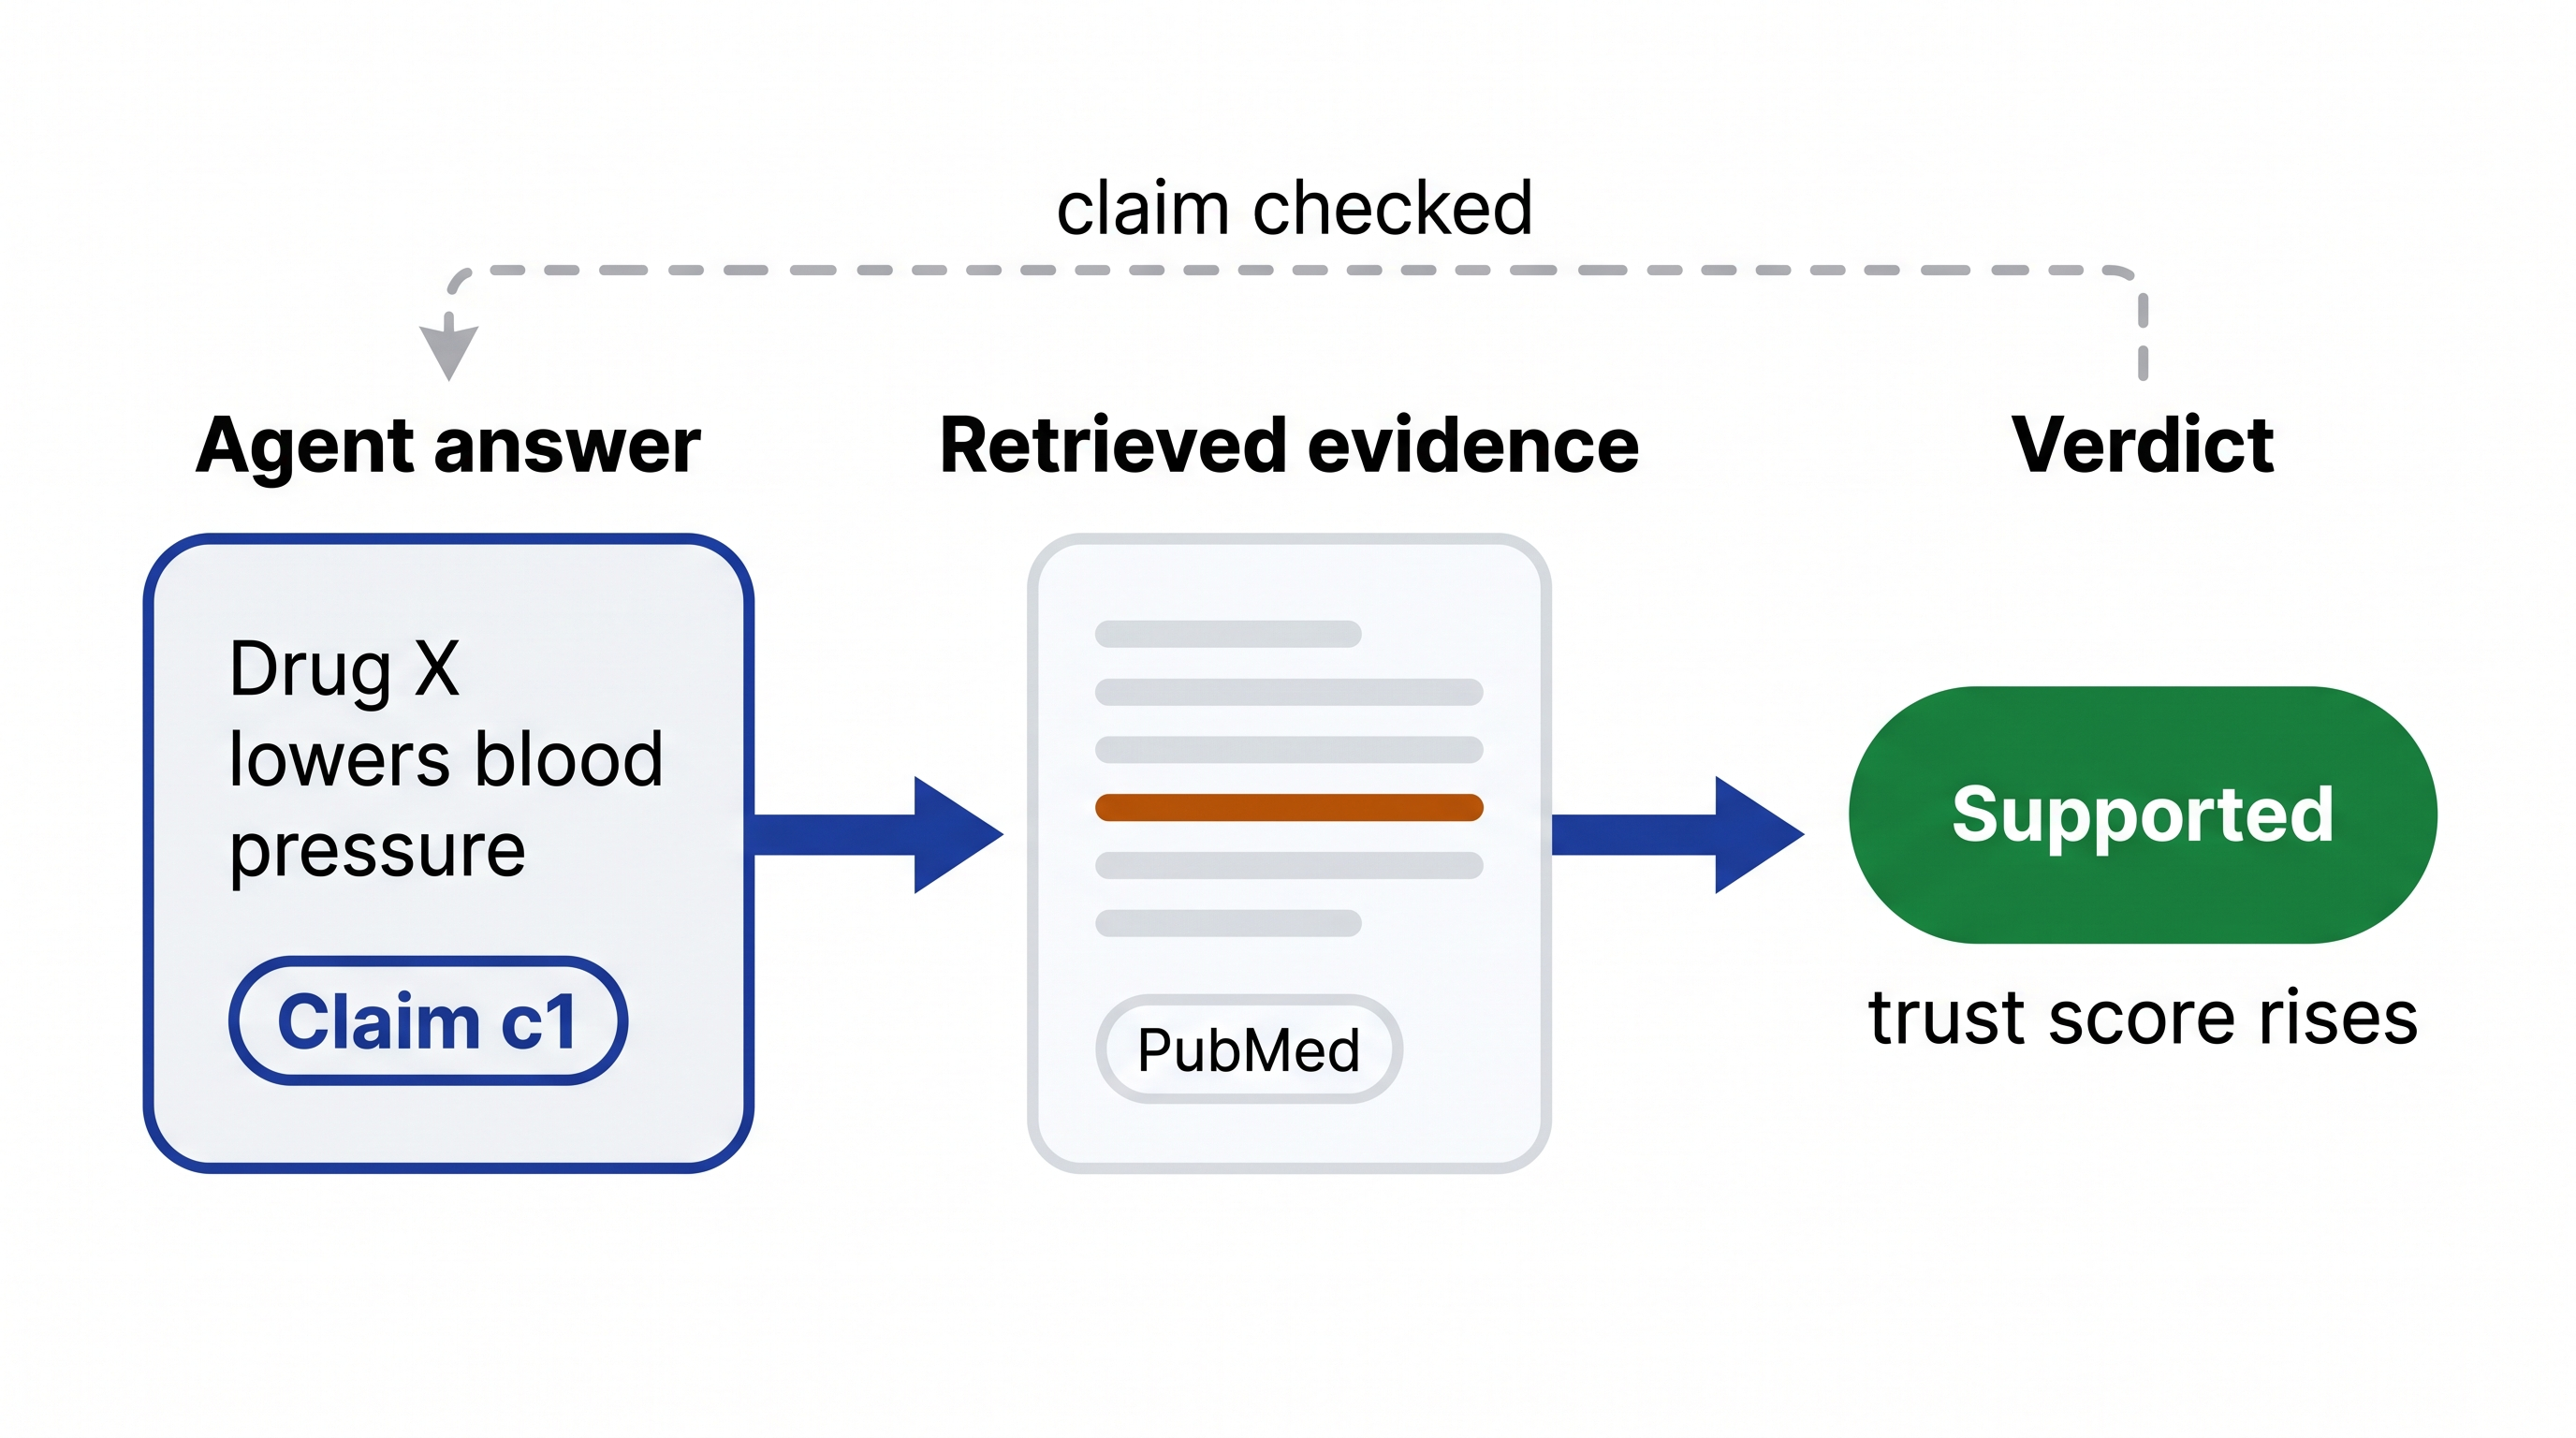
\includegraphics[width=0.80\linewidth]{fig-claim-example.png}
  \caption{Worked example of a single claim verified against a retrieved passage. The claim is marked supported, and the trust score of the agent rises for that round.}\label{fig:claim-example}
\end{figure}

\subsection{Trust Update}
The trust update converts the verdicts into a bounded influence score. Let $S_i(t)$ be the raw score of agent $i$ at round $t$. The raw score grows with the number of supported claims $V_i$ and falls with the number of contradicted claims $H_i$:
\begin{equation}\label{eq:score}
  S_i(t+1) = S_i(t) + \alpha V_i - \beta H_i
\end{equation}
where $\alpha$ and $\beta$ control the gain and the loss. The raw scores are then converted into weights. A softmax maps the raw scores into positive values, a clamp keeps each value inside the interval $[0.1, 0.9]$, and a renormalization returns the weights to the simplex:
\begin{equation}\label{eq:weights}
  T_i = \frac{\mathrm{clamp}(\mathrm{softmax}(S)_i, 0.1, 0.9)}{\sum_{j=1}^{N} \mathrm{clamp}(\mathrm{softmax}(S)_j, 0.1, 0.9)}
\end{equation}
The clamp addresses two potential failure modes. First, it ensures that no agent is muted because its weight is set to zero. Second, the clamp ensures that no single agent monopolizes the discussion by setting its weight to one. Since the renormalization equation always normalizes the weights to be equal to one, the final vote is still a weighted random selection from the agent positions. The bounded trust update equations~\eqref{eq:score} and ~\eqref{eq:weights}, which are solely based on the number of votes each agent receives, form the basis for all updates. In addition, as shown in Figure \ref{fig:trust-detail}, this represents an update trace from the number of votes received by each of the three agents to their final weights.
\begin{figure}[pos=htbp]
  \centering
  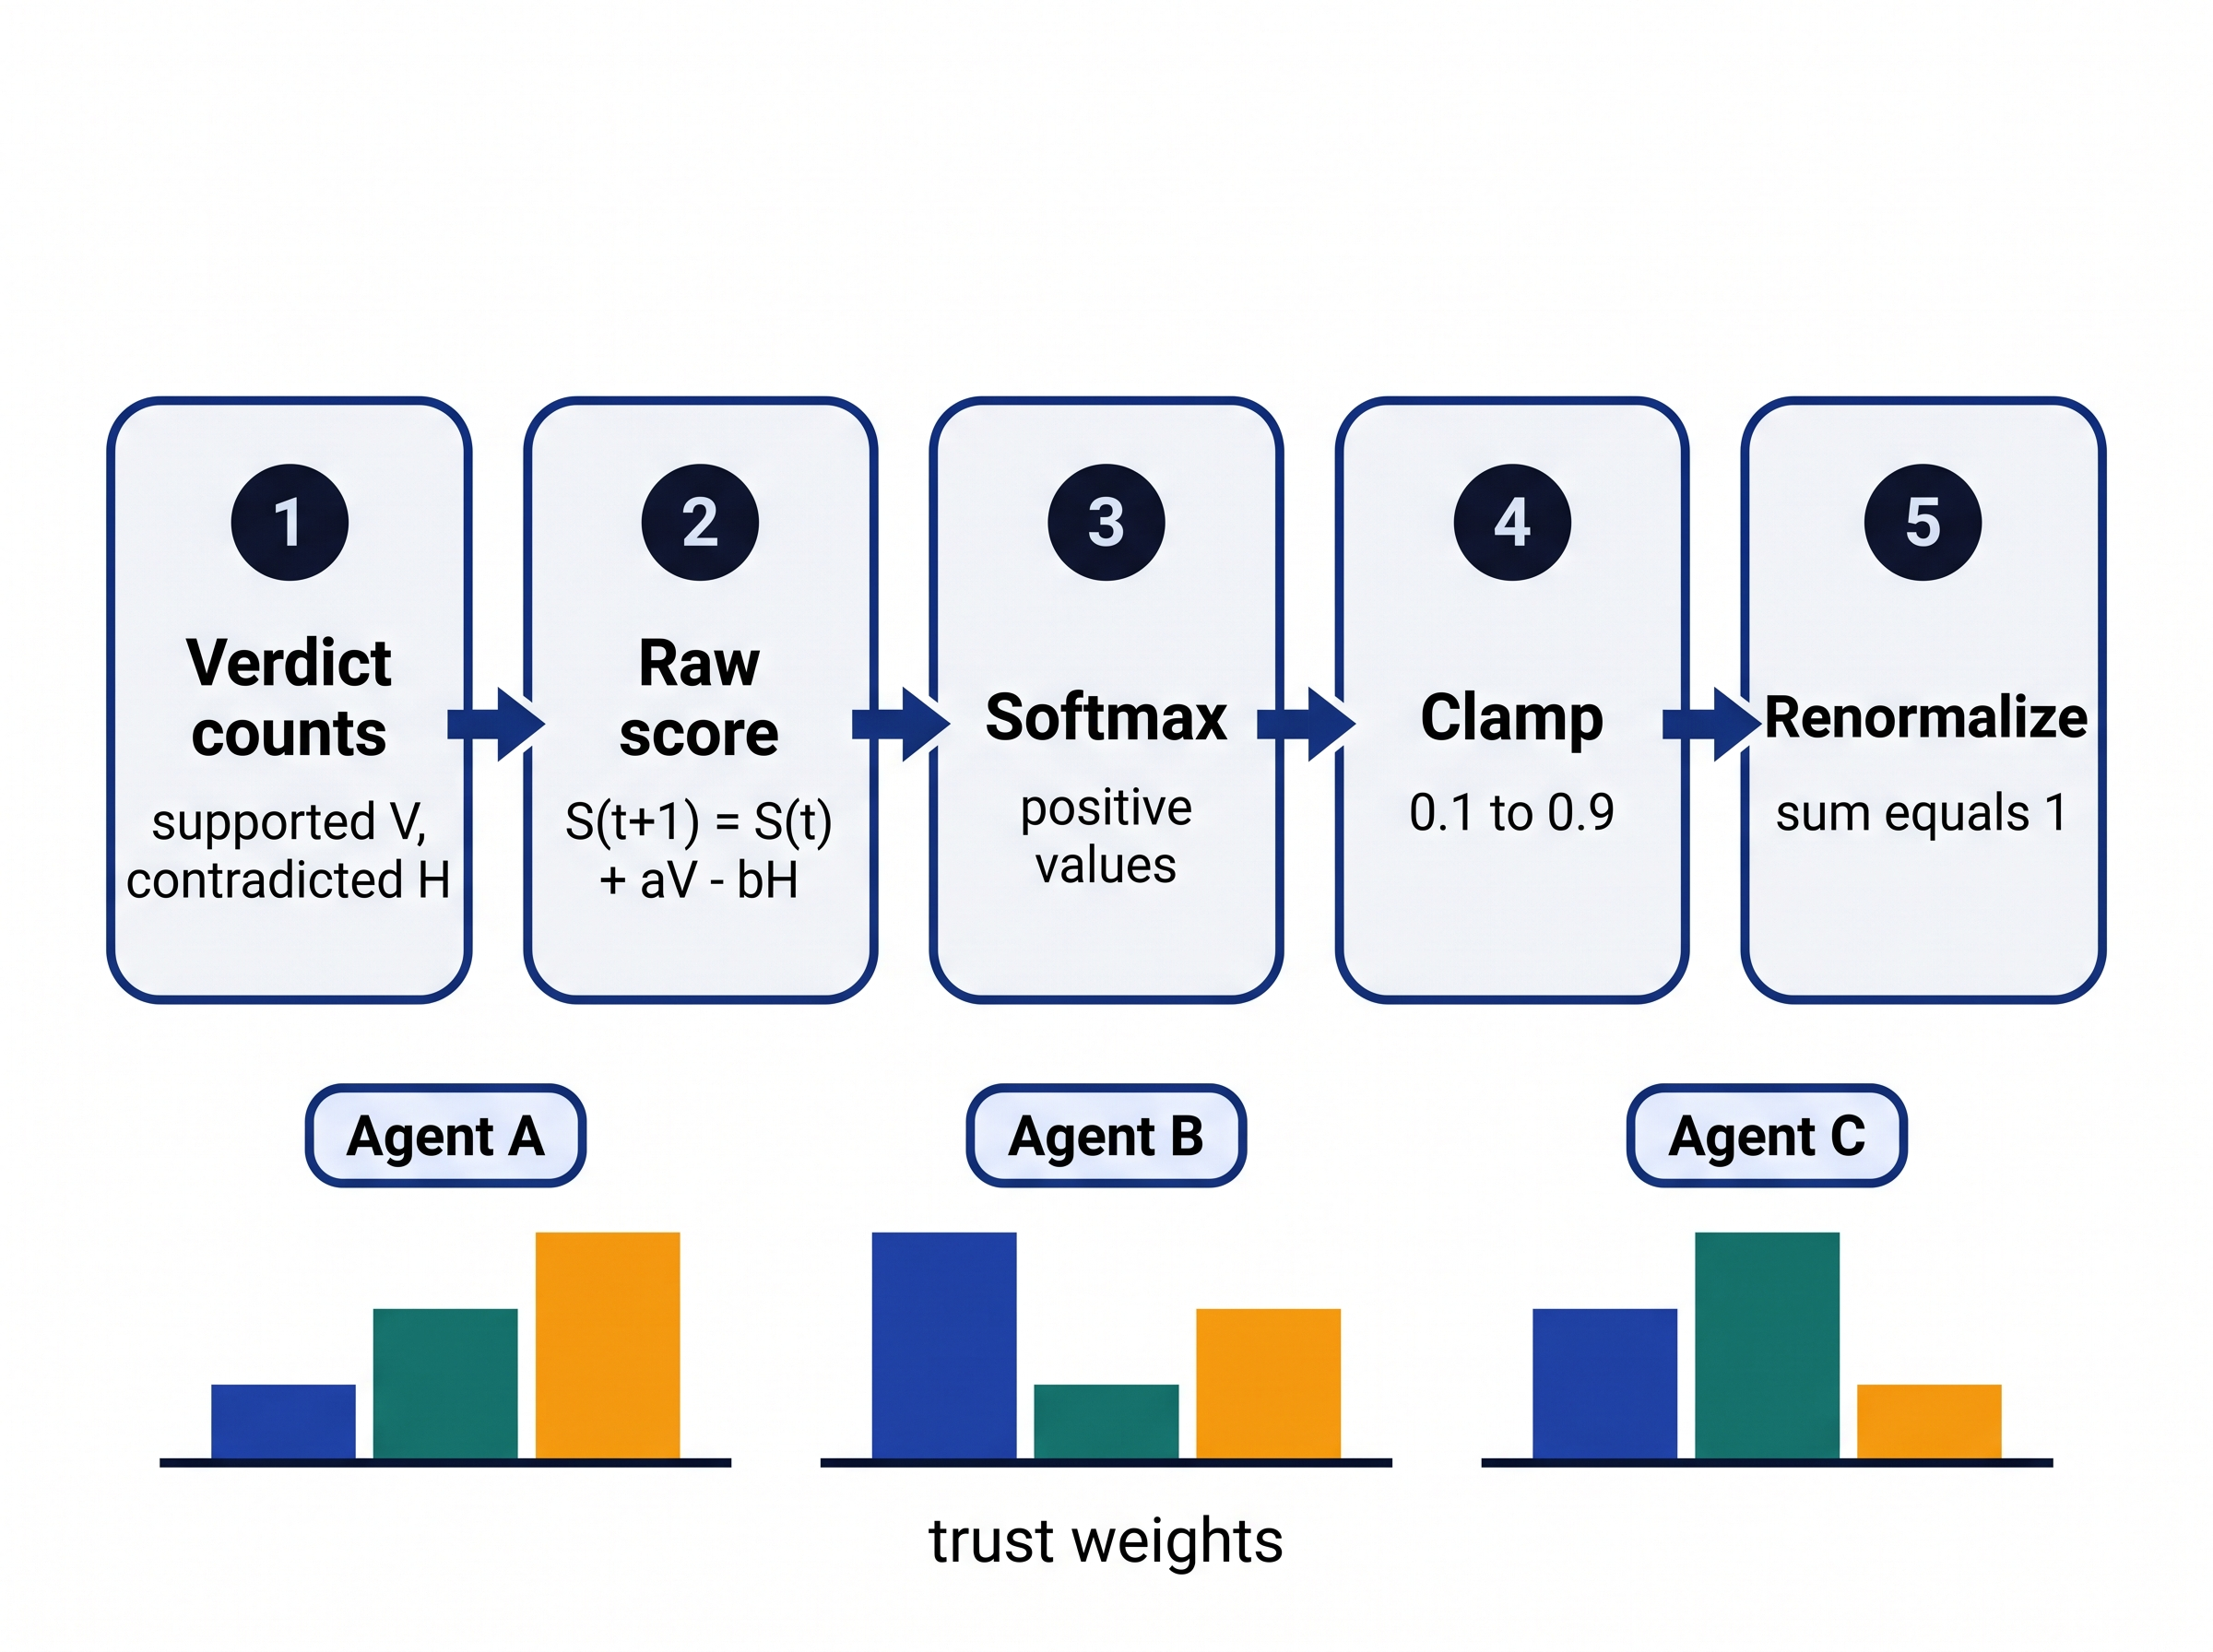
\includegraphics[width=0.58\linewidth]{fig-trust-detail.png}
  \caption{The five steps of one trust update. The verdict counts feed the raw score, and the softmax, clamp, and renormalization steps turn that score into the final trust weights of the three agents.}\label{fig:trust-detail}
\end{figure}

\subsection{Deliberation Protocol}
All rounds are in the following order; Positions, Decomposition, Retrieval, Verdicts, Trust Update. Each round of debating on a topic will call the model approximately ten times. The first or third time the model is called is to check if there is enough confidence for the gate. The next three calls are made in the first round of position taking by all parties. The last six calls are made in each of the two revision rounds. There are no model calls for claim checking, updating of trusts, injection points, nor for the aggregate at the end of each round. Agents have access to their own and other agents' positions, as well as their current trust values in both Round Two and Round Three. After Round Three the debate is over. The evaluation harness inserts an injected expert consensus at an injection point situated between Round One and Round Two. This expert consensus will contradict what is known to be correct from a minority position. No expert consensus is ever inserted during normal operation. Figure~\ref{fig:round-loop} illustrates the loop that defines how the debate proceeds through the rounds. Any agent who does not complete either the timeout or the parsing step has an inconclusive round and the debate continues with the remaining agents. Figure~\ref{fig:dataflow} illustrates the level one data flow of the debate.

\begin{figure}[pos=htbp]
  \centering
  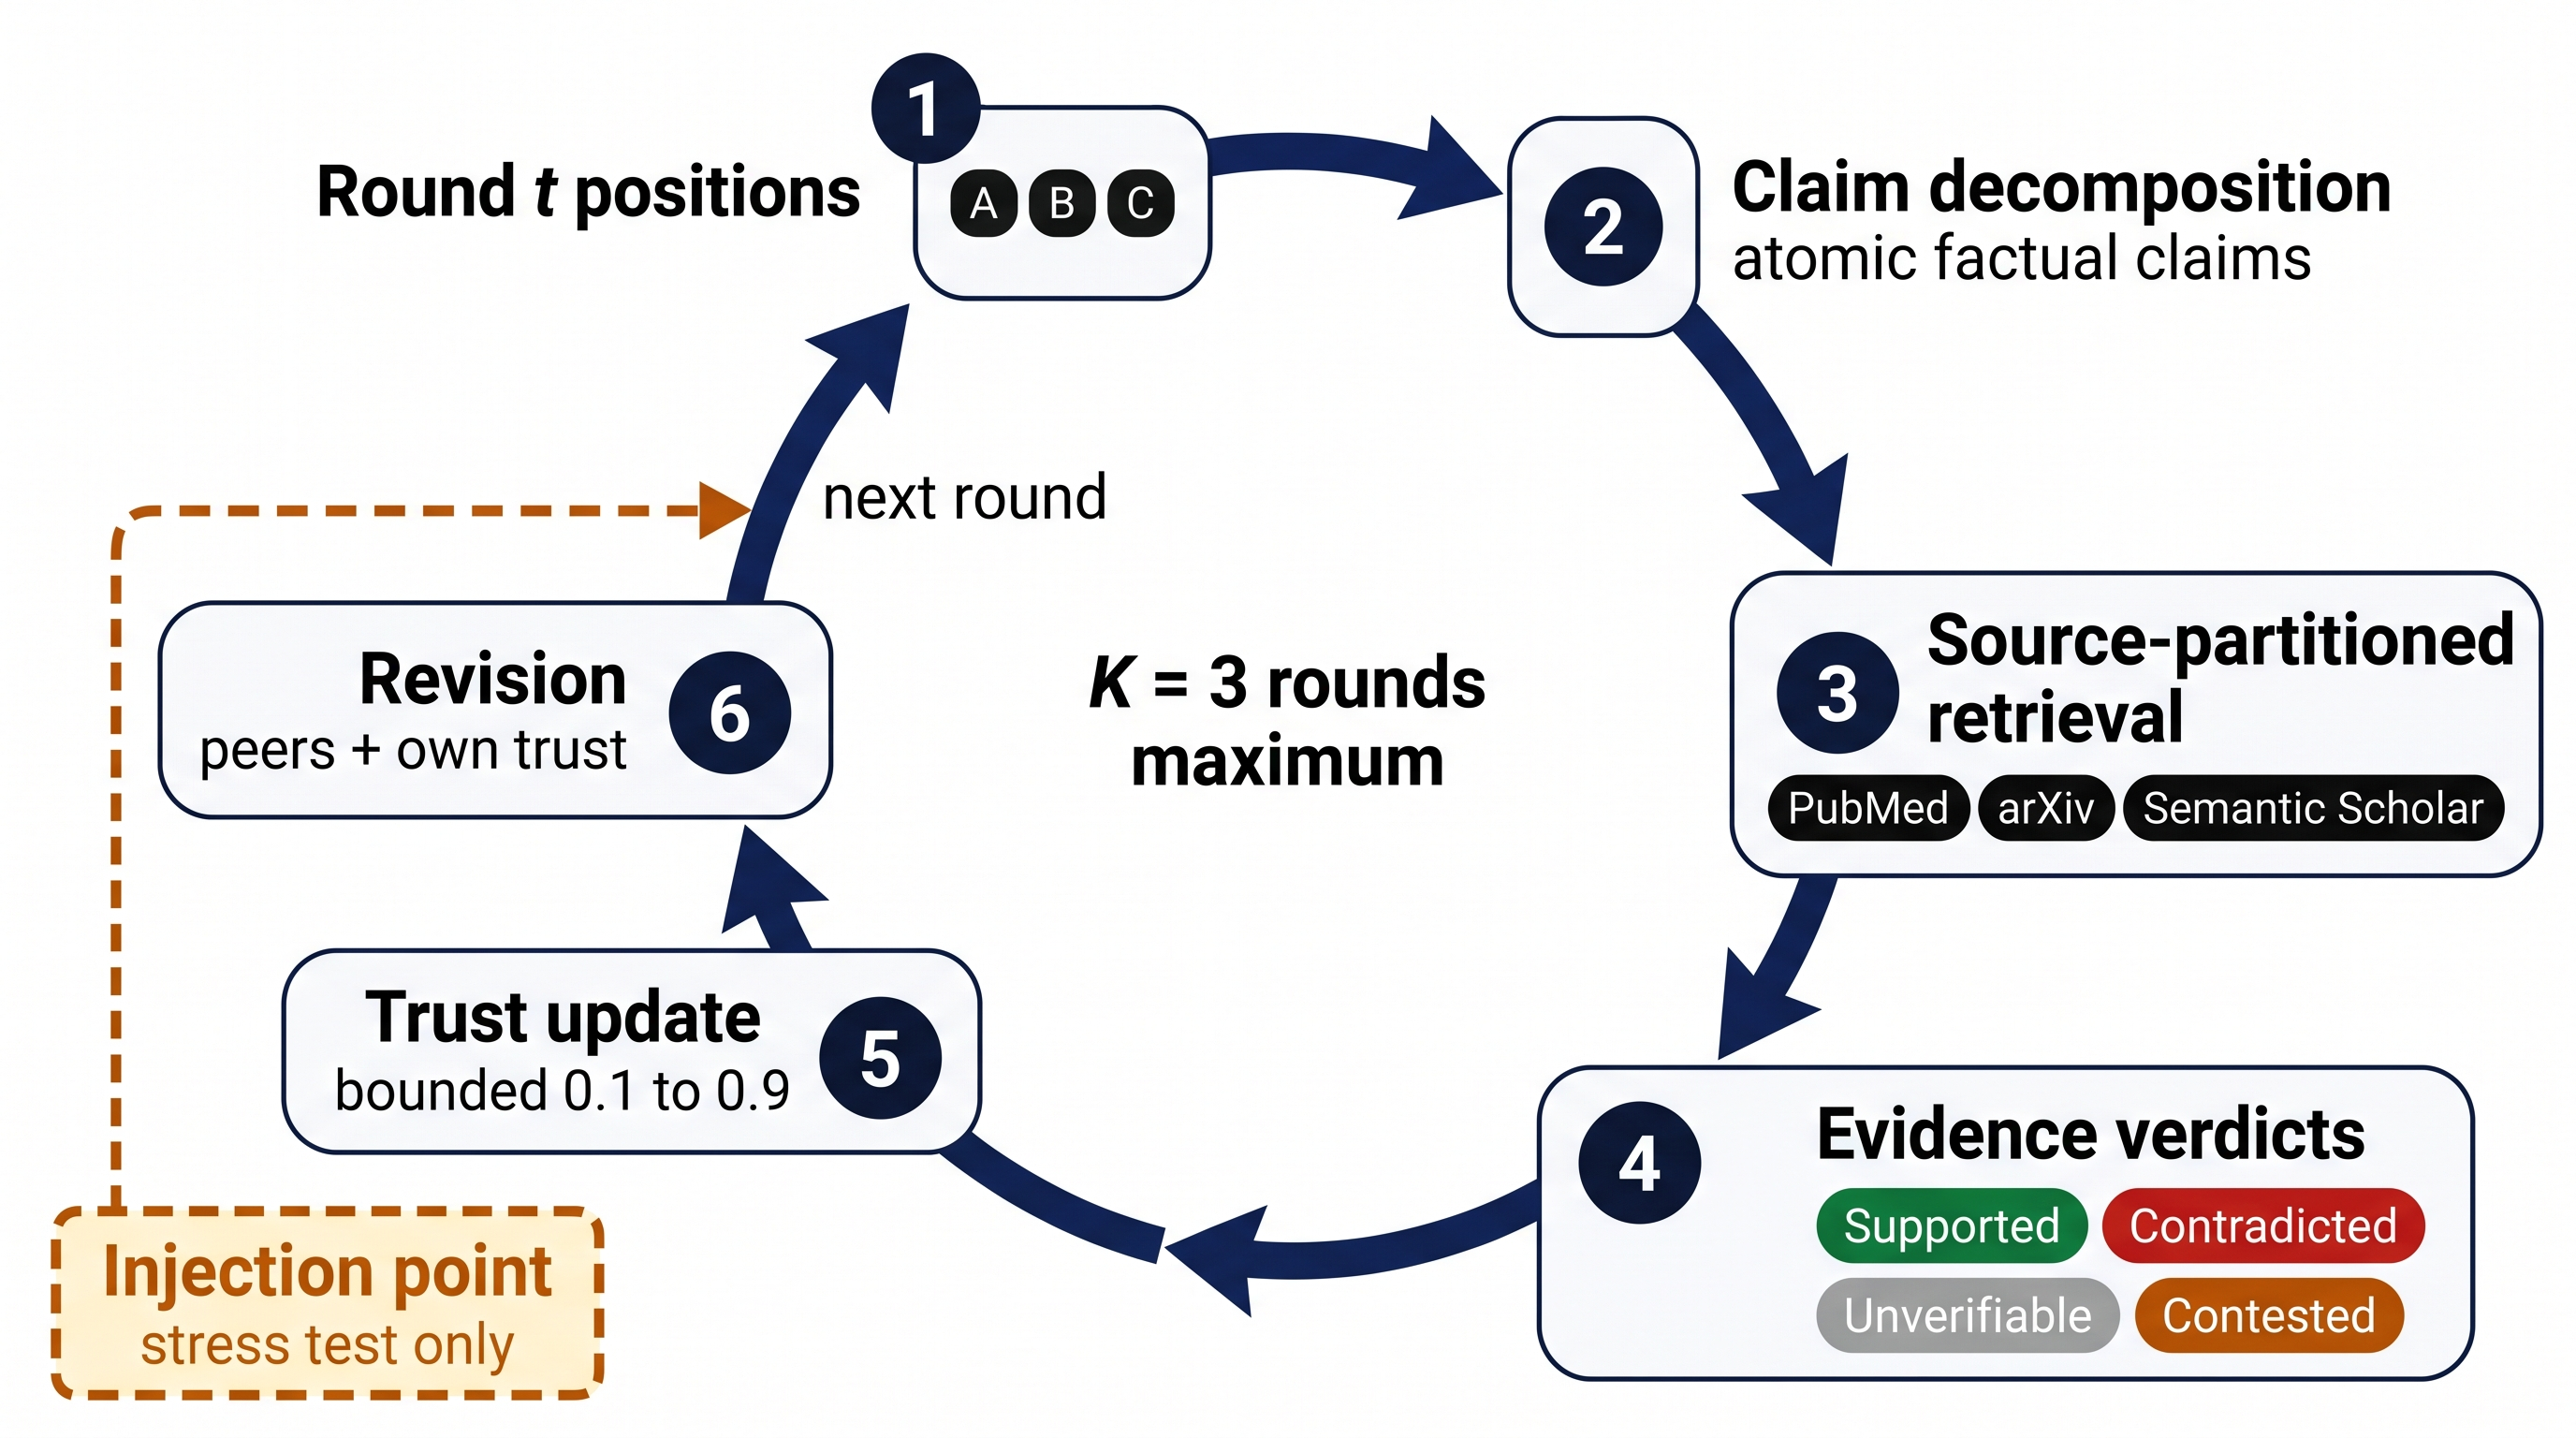
\includegraphics[width=0.88\linewidth]{fig-round-loop.png}
  \caption{The debate round loop. The six stages run in order for at most three rounds, and the injection point enters between round one and round two in the stress tests.}\label{fig:round-loop}
\end{figure}

\begin{figure}[pos=htbp]
  \centering
  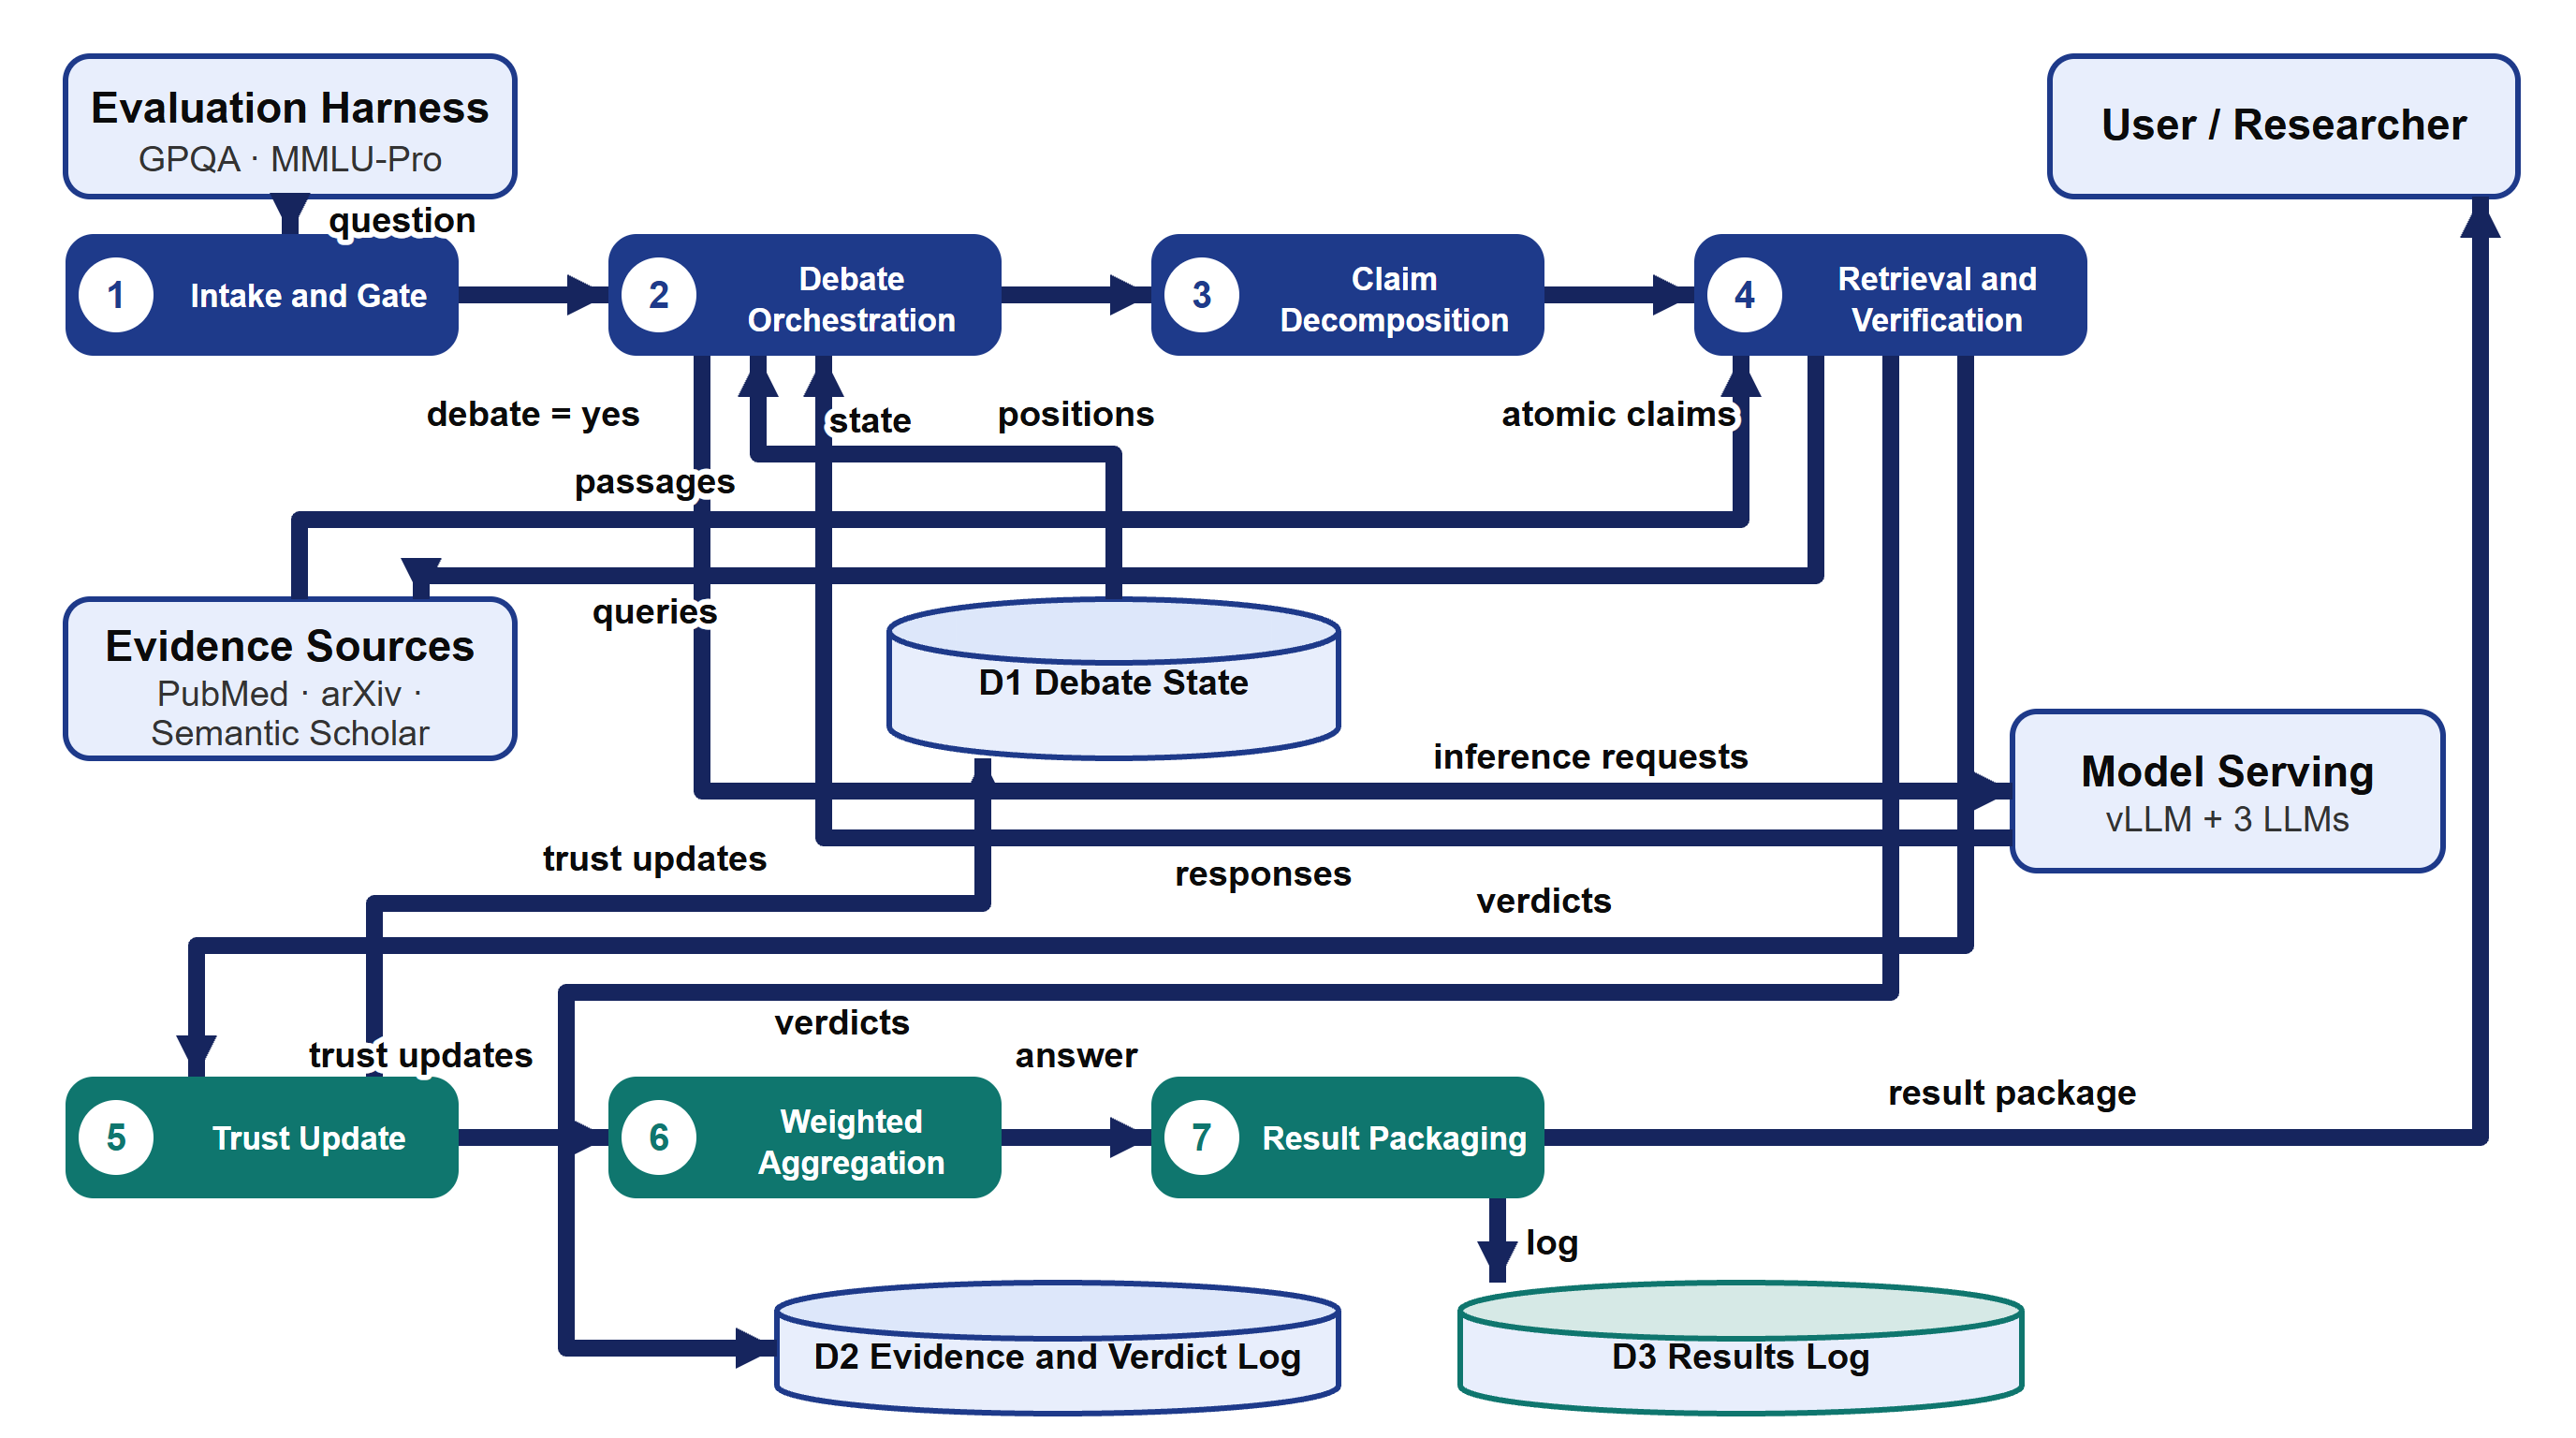
\includegraphics[width=0.88\linewidth]{fig-dataflow.png}
  \caption{Level-one data flow of the framework with the debate state, the evidence log, and the results log.}\label{fig:dataflow}
\end{figure}

\subsubsection{Trust-Weighted Aggregation}
The best answer (or the answer with the highest number of weighted votes) is determined by equation (\ref{eq:aggregate}) as follows:
\begin{equation}\label{eq:aggregate}
  a^{*} = \arg\max_{a} \sum_{i:\, p_i = a} T_i
\end{equation}
In this equation, $p_i$ represents the position (or rank) of agent $i$ in the last round, and $T_i$ is the total amount of trust assigned to it at the end of the run. Only the weighted trust of each agent is considered during the voting process; the unweighted headcount is ignored. Therefore, a small group of agents who have demonstrated strong, well-supported evidence can "outvote" an incorrect larger group. The results package will include the final answer, all cited evidence supporting or opposing it, and a record of both how much trust was allocated to each agent over time, and what decision-making path each agent followed. All agent trust allocations are recorded because they were used in calibrating the evaluation.

\clearpage

\section{Experiment}\label{sec4}

This section defines the datasets, the baselines, the metrics, the injection protocol, the serving setup, and the statistical tests that make up the evaluation.


\subsection{Datasets}

Assessment utilizes five publicly available scientifically-based question-set lists in three types of question. Two types of question are intended to generate incorrect voting behaviors from an AI, referred to as Adversarial Question Sets. A third type of question is comprised of expert-level questions (Ceiling). The last type of question, referred to as Stable Question Sets, is comprised of two question sets to determine differences in performance of the AI systems.Examples of Adversarial Question Sets include the BrokenMath and BrokenArXiv pairs. BrokenMath was built from advanced 2025 competition problems that a language model perturbs into false statements, which expert annotators then review and refine; the released benchmark contains 504 samples, of which 183 are final-answer problems and the remainder are proof-based~\cite{petrov2025brokenmath}. More recently, BrokenArXiv converts false statements from recent arXiv papers into problems and releases new problem sets monthly under a Creative Commons Attribution-ShareAlike 4.0 license ~\cite{dekoninck2026matharena}, both of which provide the agent with false premise statements that can be used to establish a sycophant agreement during a debate.The production of high quality data (ceiling) by Humanity's Last Exam and the availability of more than 2,500 questions written by experts across many subject areas, make it a viable option. Additionally, Humanity's Last Exam is free to download under Massachusetts Institute of Technology (MIT) terms. However, you must agree to use it and you may not redistribute the data ~\cite{phan2026hle}.GPQA contains approximately 450 multiple-choice graduate level questions related to biology, physics and chemistry that are available under CC BY 4.0. The study utilized the Diamond subset of GPQA that includes 198 peer-reviewed journal article questions ~\cite{rein2024gpqa}.MMLU-Pro provides students with ten answer options and requires them to explain why they chose a particular response. Like Humanity's Last Exam, MMLU-Pro is provided by MIT without charge; however, MMLU-Pro currently offers more than twelve thousand questions available across fourteen disciplines ~\cite{wang2024mmlupro}.Whereas Stable Question Sets utilize similar methods to the Main Matrix and evaluate if/when the method(s) maintain baseline levels of correctness, Adversarial Question Sets evaluate if/when the method(s) work under duress.Before entering into the pool, two pre-screening filters were applied to each set of questions. The Divergent Filter retained all questions that were answered differentially than at least two of the three agents in round one. Approximately 60--70\% of each original set passed the divergent filter for both adversarial sets. The Answer-Type Filter retained only questions where answers could be verified (i.e., multiple choice options, numbers).The main matrix draws 1,000 questions per dataset and the pilot draws 50.

\subsection{Baselines}

The performance of the Trust-Calibrated System will be compared to ten Baseline Systems in this evaluation. These ten Baseline Systems are as follows: B1 - Single Chain-of-Thought~\cite{wei2022chain}; B2 - Both Channels; B3 - Vanilla Debate Loop as described by Du et al.~\cite{du2024improving}; B4 - Debate Loop with retrieval; B5 - multiple reasoning paths sampled from a commercial model as explained by~\cite{wang2023selfconsistency}, wherein the path that has the lowest number of inconsistent responses is selected; B6 - layered pipeline as described by Wang et al.~\cite{wang2025mixture}; B7 - each question sent to large commercial model and highest percentage accurate answers across all questions used; B8 - trust calibration; B9 - implementation of iMAD from Fan et al.~\cite{fan2026imad}; and B10 - consensus agent from Pitre et al.~\cite{pitre-etal-2025-consensagent}.

These Baseline Systems directly address the two primary concerns associated with this group of studies. The first concern regarding consistency of response has been addressed through comparing B5 to the remainder of the Baseline Systems. B5 evaluates the performance of the proposed system's generation of consistent responses versus methodologies currently employed to aggregate responses. The final three Baseline Systems (B6, B9, and B10) have been compared to B6 and will provide insight into an effective methodology(ies) to aggregate responses.

Ultimately, the comparisons among these Baseline Systems will allow us to evaluate the effects of both debate and retrieval on the proposed system. Because the only difference between B1/B2 and B3/B4 were whether either included/excluded the Evidence Channel, we can assess if including the Evidence Channel in our system would benefit from its addition based upon the comparative results from evaluating B1 vs. B2, or B3 vs. B4.


\subsection{Metrics}

Four metrics can measure whether a model has produced a run. Those four metrics include answer accuracy, consensus collapse rate, minority preservation rate and evidence calibration rate. The collapse rate is the most important of those metrics for two reasons. First, it best captures the type of loss that the framework seeks to address by measuring how many times agents give up the correct answer when they receive the wrong majority vote from other agents. Second, it is an actual number (a ratio of collapse to total exposed) rather than a vague concept like ``accuracy.''

For each of the rounds in a debate assume there was a person who had the right answer to the question before the injection occurred. In addition, use E for the set of all the agents who both answered the first round correctly and were assigned the incorrect majority vote through the injection process. Use C for the set of all the agents in E who have answered differently at some point after the first round even though no additional information about the question was added during those subsequent rounds. The consensus collapse rate is then defined as:
\begin{equation}
  \mathrm{CCR} = \frac{|C|}{|E|}.
\end{equation}

\textbf{Minority Preservation Rate} --- This is also measured using debate-level data. To define this rate, consider two sets, P and D. Set D will consist of all the debates that started out with at least two different answers to the question, and P will consist of all such debates for which at least one agent gave the correct answer at the end of the debate, or if multiple agents gave the correct answer, at least one of them did so. Finally, define Minority Preservation Rate as:
\begin{equation}
  \mathrm{MPR} = \frac{|P|}{|D|}.
\end{equation}
\textbf{Evidence Calibration Rate} --- Measures how well a model's trust weights match its claimed values. At the end of a round, interpret each agent's trust weight as a degree of confidence that the agent assigns to its last answer. Compare that confidence with the proportion of time that an agent gives correct answers within the same range of confidence. Define B to be the number of ranges into which we divide confidence levels. For each range b, define nb to be the number of agents whose confidence lies in that range. Define tb to be the average trust weight among those agents whose confidence lies in that range. Define acc(b) to be the proportion of those agents in range b whose final answer is correct. Now, we can define the Expected Calibration Error~\cite{guo2017calibration} and Evidence Calibration Rate as follows:
\begin{equation}
  \mathrm{ECE} =
  \sum_{b=1}^{B}
  \frac{n_b}{N}
  \left|
  \bar{t}_b-\mathrm{acc}(b)
  \right|,
  \qquad
  \mathrm{ECR} = 1-\mathrm{ECE}.
\end{equation}



\subsection{Injection Protocol}

Six steps in order to achieve controlled pressure so as to cause a collapse of the debate via the injection protocol. Step one is when all three agents are run; questions continue to go unanswered until the divergence of the responses of the first round can be determined. In Step two, those questions which cannot verify an answer are discarded. In Step three, a fabrication of consensus based on the majority answer is created. However, this fabrication of consensus is wrong since the minority (correct answer) will have been selected by the fabrication of consensus on those questions which survived Step one. In Step four, an announcement of the fabricated ``expert'' consensus is sent out to the agents that do not accept it (those representing the correct minority). This announcement is sent after the completion of Round one but before Round two begins. No further pressure is applied to the agents subsequent to this. In Step five, the debate continues into the last three rounds consistent with the normal procedure. In Step six, the amount of abandonment is computed utilizing Equation~\eqref{eq:ccr}.

The Protocol had been validated prior to the execution of the Pilot. Samples of forty random questions were annotated and each question was labeled as either eligible or ineligible for utilization within the Protocol. The Protocol was approved if annotators agreed on eligibility for at least 0.75 using Cohen's Kappa. The Kappa statistic is described as follows:
\begin{equation}\label{eq:kappa}
  \kappa = \frac{p_o - p_e}{1-p_e},
\end{equation}
where po represents the actual proportion of agreement and pe represents the expected proportion of agreement due to pure chance.

If a Kappa value below the specified threshold exists, then the rubric for labeling is to be evaluated and altered as needed such that compliance is achieved, allowing for the Pilot to begin.


\subsection{Experimental Setup}

All models run as served inference, and no model is fine-tuned. The development stack uses Qwen3.5-9B, Gemma 4 12B, and Ministral-3-14B-Instruct-2512, and the final stack replaces them with Qwen3.6-27B, Gemma 4 26B A4B, and Mistral-Small-3.2-24B-Instruct-2506. The development stack runs on one rented RTX A6000 with 48 GB of memory. The checkpoints run at 4-bit precision, namely AWQ for Qwen and Ministral and QAT for Gemma, because the official Ministral FP8 checkpoint does not load on this card. The final stack runs on an RTX PRO 6000 Blackwell with 96 GB of memory.

Serving uses vLLM behind an OpenAI-compatible interface, with one server per agent and three servers on one card. Each server starts in sequence, and a readiness check gates the next start so that the memory profiling of one server does not disturb the others. A debate uses at most three rounds, the sampling temperature is 0.7, and each response is capped at 1{,}024 tokens. Every condition runs with three seeds, and each agent receives a seed derived from the run seed. A pilot run of ten GPQA questions on the development stack completed all three rounds for every debate, with a mean debate time of 370.8 seconds.

\subsection{Statistical Analysis}

Each condition runs with three seeds, and every reported rate carries a 95 percent confidence interval from a paired bootstrap over questions~\cite{koehn2004statistical}. The bootstrap resamples the paired question set 10{,}000 times and takes the 2.5th and 97.5th percentiles of the resampled statistic. Two conditions are compared on the same resampled questions, so the interval reflects the paired design.

The effect size uses Cohen's $d$ on the per-question outcomes:
\begin{equation}\label{eq:cohend}
  d = \frac{\bar{x}_1 - \bar{x}_2}{s_p},
\end{equation}
where $\bar{x}_1$ and $\bar{x}_2$ are the mean per-question outcomes of the two conditions and $s_p$ is the pooled standard deviation. A condition counts as an improvement only when the confidence interval of the difference stays above zero across the three seeds.

\section{Results}

\section{Conclusion}

\section*{Declarations}
\begin{itemize}
  \item \textbf{Conflicts of Interest:}  The authors declare no conflicts of interest.

  \item \textbf{Data availability:} Data will be made available on request to the corresponding
        authors.
\end{itemize}
%%%%%%%%%%%%%%%%%%%%%%%%%%%%%%%
\printcredits

\newpage
\bibliographystyle{elsarticle-num}
\nocite{*}
\bibliography{cas-refs}

\vspace{12pt}
\end{document}

